\documentclass[11pt]{article}

% ---------- Packages ----------
\usepackage[margin=1in]{geometry}
\usepackage{amsmath, amssymb, amsthm}
\usepackage{graphicx}
\usepackage{enumitem}
\usepackage{tikz}
\usepackage{xcolor}
\usepackage{hyperref}
\usepackage{fancyhdr}

% ---------- Header / Footer ----------
\pagestyle{fancy}
\fancyhf{}
\fancyhead[L]{EE 513: Stochastic Systems Theory}
\fancyhead[R]{Homework Assignment 1}
\fancyfoot[C]{\thepage}

% ---------- Custom "Solution" environment ----------
\newenvironment{solution}{\par\noindent\textbf{Solution.}\ }{\par\vspace{6pt}}

% ---------- Title Info ----------
\title{EE 513: Stochastic Systems Theory \\ Fall 2026 \\ Homework Assignment 1 \\ Template generated by Claude, solutions completed by me}
\author{Andrew Bowie}
\date{Due: Tuesday, September 8, 2026}

\begin{document}

    \maketitle

    \section*{Problem 1.1}

% Network diagram (nodes 1,2,3,4 and links a,b,c,d)
% Fill in / adjust the TikZ picture below to match the figure, or replace
% with \includegraphics{} if you have an image of the network.
    \begin{center}
        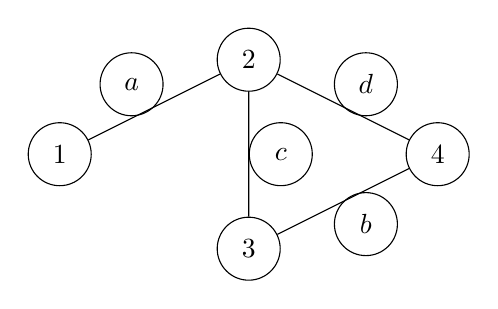
\begin{tikzpicture}[scale=1.2, every node/.style={circle, draw, minimum size=0.8cm}]
            \node (n1) at (0,1) {1};
            \node (n2) at (2,2) {2};
            \node (n3) at (2,0) {3};
            \node (n4) at (4,1) {4};

            \draw (n1) -- (n2) node[midway, above left] {$a$};
            \draw (n2) -- (n4) node[midway, above right] {$d$};
            \draw (n2) -- (n3) node[midway, right] {$c$};
            \draw (n3) -- (n4) node[midway, below right] {$b$};
        \end{tikzpicture}
    \end{center}

    \begin{enumerate}[label=(\alph*)]

    \item Construct an appropriate probability model $(S, F, P)$ with sixteen sample points $\xi$, each representing a state of the network. Specify $S$, $F$, and $P$.

    \begin{solution}

        For ease of description, a specific $\xi_a = 1$ if the link is available and $\xi_a = 0$ implies the link is not available.
        $S = \big\{(\xi_a, \xi_b, \xi_c, \xi_d) : \xi_i \in \{0, 1\}, i \in (a, b, c, d)\big\}$ \\
        $F = \big\{A: A \subseteq S \big\}$ $|F| = 2^{16} = 65536$ Since $|S| = 16$\\
        $P(\{\xi\}) = p^{n(\xi)}(1- p)^{4 - n(\xi)}$ where $n(\xi) = \xi_a + \xi_b + \xi_c + \xi_d$

    \end{solution}

    \item Let $A = \{\xi : \text{node-1 and node-4 can communicate}\}$. Calculate $P(A)$.

    \begin{solution}

        This is all $\xi$ such that a path exists between node-1 and node-4.
        Examining the graph, it appears that there are two paths it can take. $a \rightarrow c \rightarrow b$ OR $a \rightarrow d$.
        That is $B = \{(1, 1, 1, x): x \in \{0, 1\}\}$ and $C = \{(1, x, x, 1): x \in \{0, 1\}\}$.
        Therefore, $P(B \cup C) = P(B) + P(C) - P(B \cap C)$ \\
        Individually,
        \[P(B) = P(\{1, 1, 1, 0\}) + P(\{1, 1, 1, 1\}) = p^{3}(1-p) + p^4\] \\
        \[P(C) = P(\{1, 0, 0, 1\}) + P(\{1, 0, 1, 1\}) + P(\{1, 1, 0, 1\}) + P(\{1, 1, 1, 1\}) = p^2(1 - p)^2 + 2(p^3(1 - p)) + p^4\] \\
        \[P(B \cap C) = P(\{1, 1, 1, 1\}) = p^4\]
        Together,
        \begin{align}
            P(B \cup C) &= p^{3}(1-p) + p^4 + p^2(1 - p)^2 + 2(p^3(1 - p)) + p^4 - p^4\\
            &= p^2 + p^3 - p^4
        \end{align}

    \end{solution}

    \item Let $B = \{\xi : \text{node-2 and node-3 can communicate}\}$. Calculate $P(B)$.

    \begin{solution}

        This is all $\xi$ such that a path exists between node-2 and node-3.
        Examining the graph, it appears that there are two paths it can take. $c$ OR $d \rightarrow b$.
        That is $C = \{(x, x, 1, x): x \in \{0, 1\}\}$ and $D = \{(x, 1, x, 1): x \in \{0, 1\}\}$.
        Therefore, $P(C \cup D) = P(C) + P(D) - P(C \cap D)$ \\
        Individually,
        \[P(C) = p^4 + 3(p^3(1 - p)) + 3(p^2(1 - p)^2) + p(1-p)^3 = p]\] \\
        \[P(D) = p^4 + 2(p^3(1 - p)) + p^2(1-p)^2 = p^2\] \\
        \[P(C \cap D) = p^4 + p^3(1 - p) = p^3]\]
        Together,
        \begin{align}
            P(C \cup D) &= p + p^2 - p^3\\
        \end{align}

    \end{solution}

    \item Calculate $P(A \cap B)$. How many sample points of $S$ does the event $\{\xi : A \cap B\}$ contain? Are the events $A$ and $B$ statistically independent?

    \begin{solution}

        That is to say that nodes 1 and 4 can communicate, AND nodes 2 and 3 can communicate.
        \[A \cap B = \big\{\{1, 0, 1, 1\}, \{1, 1, 1, 1\}, \{1, 1, 1, 0\}, \{1, 1, 0, 1\}\big\}\] \\
        \[P(A \cap B) = 3(p^3(1-p)) + p^4 = 3p^3 - 2p^4\]
        To say that the events are statistically independent is to say that
        \begin{align}
            P(A \cap B) &= P(A)P(B)\\
            &= (p^2 + p^3 - p^4)(p + p^2 - p^3) \\
            &= p^3 + p^4 - p^5 + p^4 + p^5 - p^6 - p^5 - p^6 + p^7 \\
            &= p^3 + 2p^4 - p^5 - 2p^6 + p^7
        \end{align}
        This is clearly not the case, these events are statistically dependent.

    \end{solution}

    \item Show that
    \[
        P(A) = p\, P(A \mid \text{link-c available}) + (1-p)\, P(A \mid \text{link-c not available}).
    \]
    Use this formula to recalculate $P(A)$ by inspection.

    \begin{solution}

        Instead of finding individual probabilities, we can use the definition of conditional probability.
        Keep in mind that, by definition, $P(\text{link-c available}) = p$ and $P(\text{link-c not available}) = 1 - p$.
        \[p\, P(A \mid \text{link-c available}) = p\, \frac{P(A \cap \text{link-c available})}{p} = P(A \cap \text{link-c available})\]
        Likewise,
        \[(1-p)\, P(A \mid \text{link-c not available}) = (1-p)\, \frac{P(A \cap \text{link-c not available})}{1-p} = P(A \cap \text{link-c not available})\]
        Now we can simplify,
        \[P(A) = P(A \cap \text{link-c available}) + P(A \cap \text{link-c not available})\]
        Given $A \cap \text{link-c available}$ and $A \cap \text{link-c not available}$ and the events being mutually exclusive,
        \[(A \cap \text{link-c available}) \cup (A \cap \text{link-c not available}) = A\]
        Therefore,
        \[P(A) = p\, P(A \mid \text{link-c available}) + (1-p)\, P(A \mid \text{link-c not available})\] \\
        To confirm that these are equal by inspection, first lets look at $P(A \mid \text{link-c available})$
        Given that link c is available in the network,
        \[P(A \mid \text{link-c available}) = 2p^2(1-p) + p^3\] \\
        \[P(A \mid \text{link-c not available}) = p^2(1-p) + p^3\]
        By our found defintion,
        \begin{align}
            P(A) &= p(2p^2(1-p) + p^3) + (1 - p)(p^2(1-p) + p^3) \\
            &= 2p^3(1-p) + p^4 + p^2(1-p)^2 + p^3(1-p) \\
            &= -p^4 + p^3 + p^2
        \end{align}
        Which is the same as our original finding of A.

    \end{solution}

    \item Prove that $P(A)$ would be increased by moving link-c between node-1 and node-2 rather than between node-2 and node-3.

    \begin{solution}

    \end{solution}

    \end{enumerate}

    \newpage
    \section*{Problem 1.2}

    Let $A_1, A_2, \ldots, A_N$ be $N$ events defined on some probability space. Prove that
    \[
        P\left(\bigcup_{n=1}^{N} A_n\right) = \sum_{1 \le i \le N} P(A_i) - \sum_{1 \le i < j \le N} P(A_i \cap A_j) + \sum_{1 \le i < j < k \le N} P(A_i \cap A_j \cap A_k) - \cdots \pm P(A_1 \cap A_2 \cap \cdots \cap A_N).
    \]
    \emph{Hint: Prove the statement by induction.}

    \begin{solution}

    \end{solution}

    \newpage
    \section*{Problem 1.3}

    A random experiment $A$ has $N$ mutually exclusive outcomes $A_1, A_2, \ldots, A_N$, and random experiment $B$ has $M$ mutually exclusive outcomes $B_1, B_2, \ldots, B_M$. Establish Bayes' rule,
    \[
        \Pr(B_m \mid A_n) = \frac{\Pr(A_n \mid B_m)\Pr(B_m)}{\sum_{i=1}^{M} \Pr(A_n \mid B_i)\Pr(B_i)}.
    \]

    \begin{solution}

    \end{solution}

    \newpage
    \section*{Problem 1.4}

    A homogeneous stick of unit length is broken at two points. What is the probability that a triangle can be formed from the three pieces?

    \begin{solution}

    \end{solution}

    \newpage
    \section*{Problem 1.5}
    \emph{(Papoulis, based on Problem 4-21, p. 85)}

    The probability of heads of a random coin is a RV $p$ uniform in the interval $(0,1)$.

    \begin{enumerate}[label=(\alph*)]

    \item Find $P\{0.3 \le p \le 0.7\}$.

    \begin{solution}

    \end{solution}

    \item The coin is tossed 10 times and heads shows 6 times. Find the a posteriori probability that $p$ is between 0.3 and 0.7.

    \begin{solution}

    \end{solution}

    \end{enumerate}

    \newpage
    \section*{Problem 1.6}
    \emph{(based on Problem 2.97 on page 91, Leon-Garcia'06)}

    A block of 50 bits is transmitted over a binary communication channel with probability of bit error $p = 10^{-2}$.

    \begin{enumerate}[label=(\alph*)]

    \item If the block has 2 or fewer errors then the receiver accepts the block. Find the probability that the block is accepted.

    \begin{solution}

    \end{solution}

    \item If the block has more than 2 errors, then the block is retransmitted. Find the probability that $M$ retransmissions are required.

    \begin{solution}

    \end{solution}

    \end{enumerate}

    \newpage
    \section*{Problem 1.7}

    \begin{enumerate}[label=(\alph*)]

    \item The continuous random variable $X$ has a \emph{Laplacian} probability density function
    \[
        f_X(x) = a e^{-b|x|}, \qquad -\infty < x < +\infty,
    \]
    where $a$ and $b$ are constants. What is the relationship between $a$ and $b$? Determine and plot the cumulative probability distribution function (cdf) of $X$ for $a = 1/2$.

    \begin{solution}

    \end{solution}

    \item Repeat part (a) if $X$ has the \emph{Cauchy} probability density
    \[
        f_X(x) = \frac{a}{b^2 + x^2}.
    \]

    \begin{solution}

    \end{solution}

    \end{enumerate}

    \newpage
    \section*{Problem 1.8}

    The cumulative distribution function (cdf) $F_X(x)$ for a normal random variable with probability density
    \[
        f_X(x) = \frac{1}{\sqrt{2\pi}} e^{-x^2/2}, \qquad -\infty < x < +\infty,
    \]
    is not expressible in elementary functions, but it is extensively tabulated (see, for example, A. Abramowitz and I. Stegun, \emph{Handbook of Mathematical Functions}) and can be readily evaluated numerically on a computer. Even so, it is useful from both an analytical and computational viewpoint to have bounds and approximate expressions for the distribution function. For this purpose, define the Q-function in terms of the probability distribution function according to
    \[
        Q(x) = 1 - F_X(x) = \int_x^{+\infty} \frac{1}{\sqrt{2\pi}} e^{-y^2/2}\, dy.
    \]

    \begin{enumerate}[label=(\alph*)]

    \item Establish the following inequalities for $x > 0$:
    \[
        \frac{1}{x\sqrt{2\pi}}\left(1 - \frac{1}{x^2}\right) e^{-x^2/2} < Q(x) < \frac{1}{x\sqrt{2\pi}} e^{-x^2/2}.
    \]
    \emph{Hint: express the Q-function as}
    \[
        Q(x) = \frac{1}{\sqrt{2\pi}} \int_x^{+\infty} \left(\frac{1}{y}\right) \left(y e^{-y^2/2}\right) dy
    \]
    \emph{and integrate by parts. Use repeated application of integration by parts.}

    \begin{solution}

    \end{solution}

    \item Draw a graph of the Q-function and its upper and lower bounds in part (a). For what values of $x$ are the bounds tight?

    \begin{solution}

        % Suggested: generate the plot in Python/MATLAB and include it here, e.g.
        % 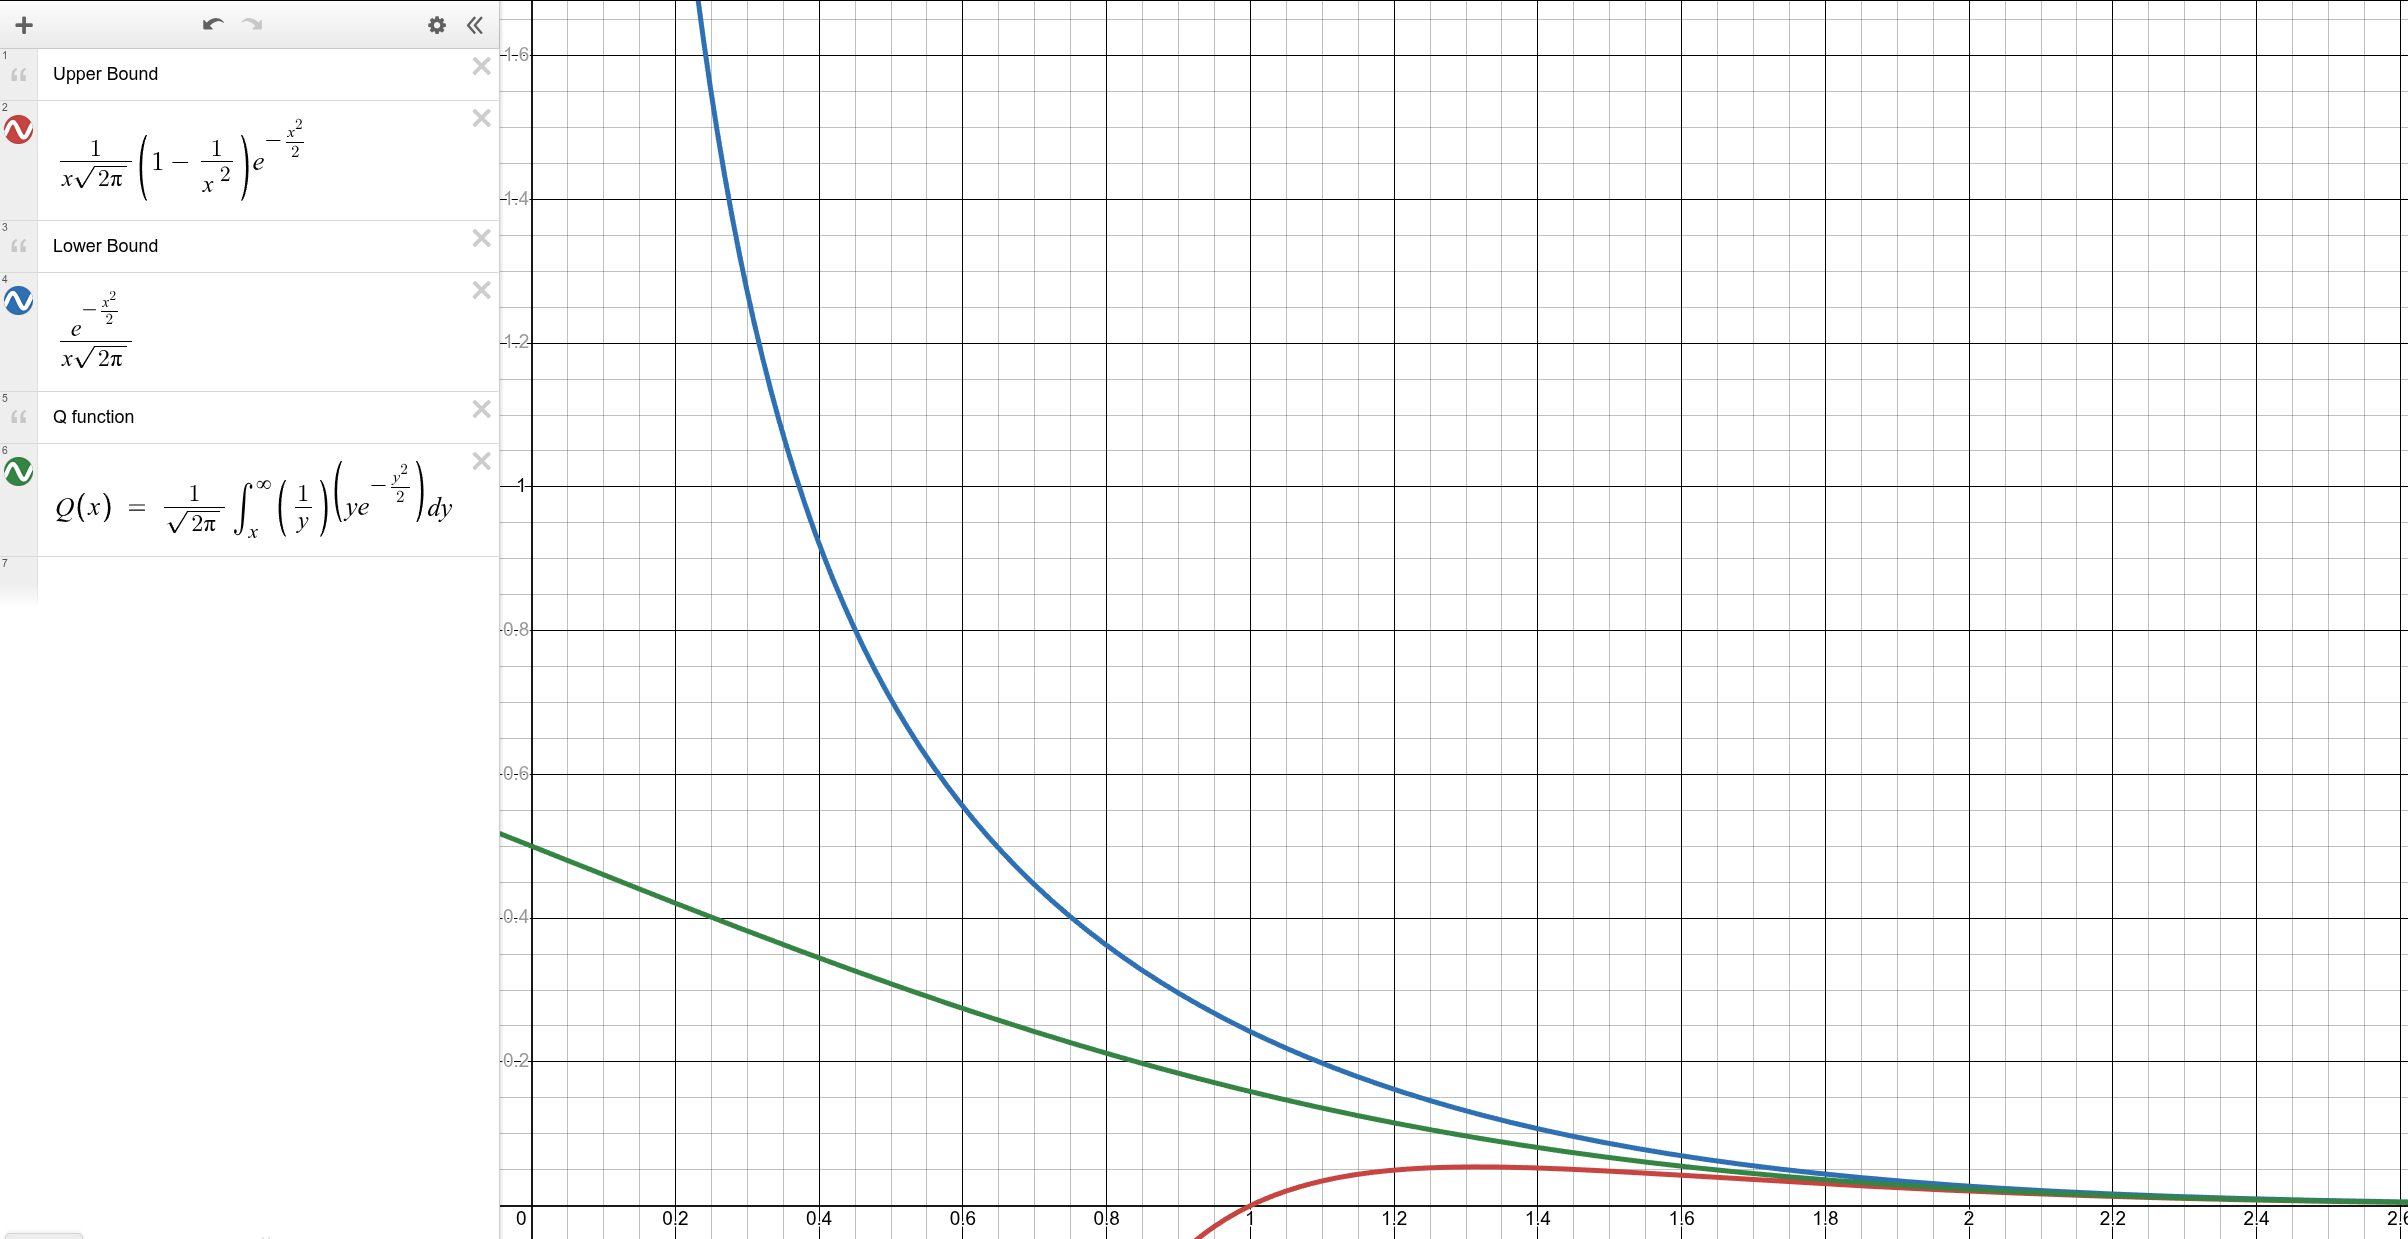
\includegraphics[width=0.7\textwidth]{q_function_bounds.png}

    \end{solution}

    \end{enumerate}

\end{document}